% 61-16(61쪽) — 도함수 y=f'(x) 의 그래프(사차 모양 · 왼쪽 x절편은 −4 와 −3 사이 · x=0 에서 x축에 접함 · 오른쪽 x절편 3). 스캔 화질이 낮아 TikZ 로 다시 그림.
% 원문에 있는 것만: 눈금 숫자 −4 −3 −1 2 3 4 · 라벨 O, x, y, y=f'(x) · 안내 파선(−4 와 4 는 축에서 아래로 곡선까지, −3 · −1 · 2 는 축에서 위로 곡선까지).
% 눈금 −3 · −1 · 2 · 4 는 보기 ㄱ~ㄹ 의 구간 끝이고 x절편이 아니다. 원문의 왼쪽 x절편은 −4 보다 오른쪽(약 −3.7)에 있으므로 그대로 옮긴다 — 여기를 −4 로 그리면 보기 ㄱ 의 참거짓이 뒤집힌다.
% 곡선은 식이 주어진 그래프가 아니라 원문 모양을 재어 지나는 점을 smooth 로 이었다. y 값은 원문 비율만 맞춘 것이고 눈금이 없다.
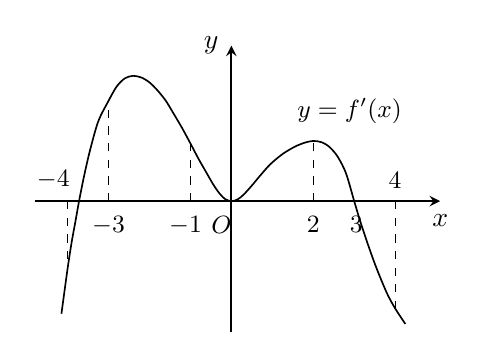
\begin{tikzpicture}[x=0.52cm, y=0.52cm, line width=0.5pt]
  \draw[->, >=stealth, line width=0.7pt] (-4.8,0) -- (5.1,0) node[below=1pt] {$x$};
  \draw[->, >=stealth, line width=0.7pt] (0,-3.2) -- (0,3.8) node[left=1pt] {$y$};
  \node[below=2pt, font=\small] at (-0.24,0) {$\pt{O}$};
  % 안내 파선(원문)
  \draw[dashed, line width=0.35pt] (-4,0) -- (-4,-1.65);
  \draw[dashed, line width=0.35pt] (-3,0) -- (-3,2.45);
  \draw[dashed, line width=0.35pt] (-1,0) -- (-1,1.41);
  \draw[dashed, line width=0.35pt] (2,0) -- (2,1.47);
  \draw[dashed, line width=0.35pt] (4,0) -- (4,-2.62);
  % 그래프
  \draw[line width=0.6pt, smooth] plot coordinates {(-4.15,-2.75) (-4.00,-1.65) (-3.90,-1.00) (-3.80,-0.45) (-3.72,0) (-3.60,0.60) (-3.45,1.25) (-3.25,1.95) (-3.00,2.45) (-2.80,2.80) (-2.60,3.00) (-2.40,3.06) (-2.20,3.02) (-2.00,2.90) (-1.80,2.70) (-1.60,2.45) (-1.40,2.12) (-1.20,1.78) (-1.00,1.41) (-0.80,1.03) (-0.60,0.68) (-0.45,0.42) (-0.30,0.20) (-0.15,0.05) (0,0) (0.15,0.04) (0.30,0.16) (0.50,0.38) (0.70,0.62) (0.95,0.90) (1.25,1.15) (1.55,1.33) (1.80,1.43) (2.00,1.47) (2.20,1.44) (2.40,1.32) (2.60,1.08) (2.80,0.68) (3.00,0) (3.15,-0.50) (3.35,-1.10) (3.55,-1.65) (3.80,-2.25) (4.00,-2.62) (4.25,-3.00)};
  % 눈금 라벨(원문 자리 그대로: −4 와 4 는 축 위, −3 · −1 · 2 · 3 은 축 아래)
  \node[above=1pt, font=\small] at (-4.35,0) {$-4$};
  \node[below=2pt, font=\small] at (-3,0) {$-3$};
  \node[below=2pt, font=\small] at (-1.12,0) {$-1$};
  \node[below=2pt, font=\small] at (2,0) {$2$};
  \node[below=2pt, font=\small] at (3.05,0) {$3$};
  \node[above=1pt, font=\small] at (4,0) {$4$};
  \node[right=1pt, font=\small] at (1.3,2.2) {$y=f'(x)$};
\end{tikzpicture}
